% DeepLab architecture variants — three-panel comparison
% (a) Spatial Pyramid Pooling  → DeepLabv3
% (b) Encoder-Decoder          → U-Net
% (c) Encoder-Decoder + Atrous → DeepLabv3+
%
% Compile:  pdflatex deeplab_variants.tex

\documentclass[tikz, border=12pt]{standalone}
\usepackage{tikz}
\usetikzlibrary{arrows.meta, positioning, calc, fit, backgrounds}

\definecolor{cenc} {RGB}{ 59, 120, 196}
\definecolor{cdec} {RGB}{ 46, 155,  82}
\definecolor{cbn}  {RGB}{123,  79, 166}
\definecolor{caspp}{RGB}{142,  68, 173}
\definecolor{cskip}{RGB}{230, 126,  34}
\definecolor{cpool}{RGB}{192,  57,  43}
\definecolor{cup}  {RGB}{ 39, 174,  96}
\definecolor{cimg} {RGB}{189, 195, 199}
\definecolor{cpred}{RGB}{ 39, 174,  96}
\definecolor{cpanel}{RGB}{240, 244, 255}

\tikzset{
  blk/.style  = {rectangle, draw=white, line width=0.4pt,
                 text=white, font=\scriptsize, text centered,
                 minimum width=#1, minimum height=0.62cm},
  blk/.default = 2.4cm,
  imgblk/.style = {rectangle, fill=cimg, draw=gray!50, line width=0.5pt,
                   text=black, font=\scriptsize,
                   minimum width=2.4cm, minimum height=0.62cm},
  >=Stealth
}

% Helper: vertical stack of n feature-scale rectangles (shrinking upward)
% Usage: \featstack{<base x>}{<base y>}{<fill colour>}{<n levels>}
\newcommand{\featstack}[4]{%
  \foreach \k in {1,...,#4} {%
    \pgfmathsetmacro{\sc}{1.0 - 0.12*(\k-1)}%
    \pgfmathsetmacro{\ht}{0.44 * \sc}%
    \pgfmathsetmacro{\yw}{2.2 * \sc}%
    \pgfmathsetmacro{\ypos}{#2 + (\k-1)*0.50}%
    \node[rectangle, fill=#3, draw=white, line width=0.3pt,
          minimum width=\yw cm, minimum height=\ht cm]
      at (#1, \ypos cm) {};%
  }%
}

\begin{document}
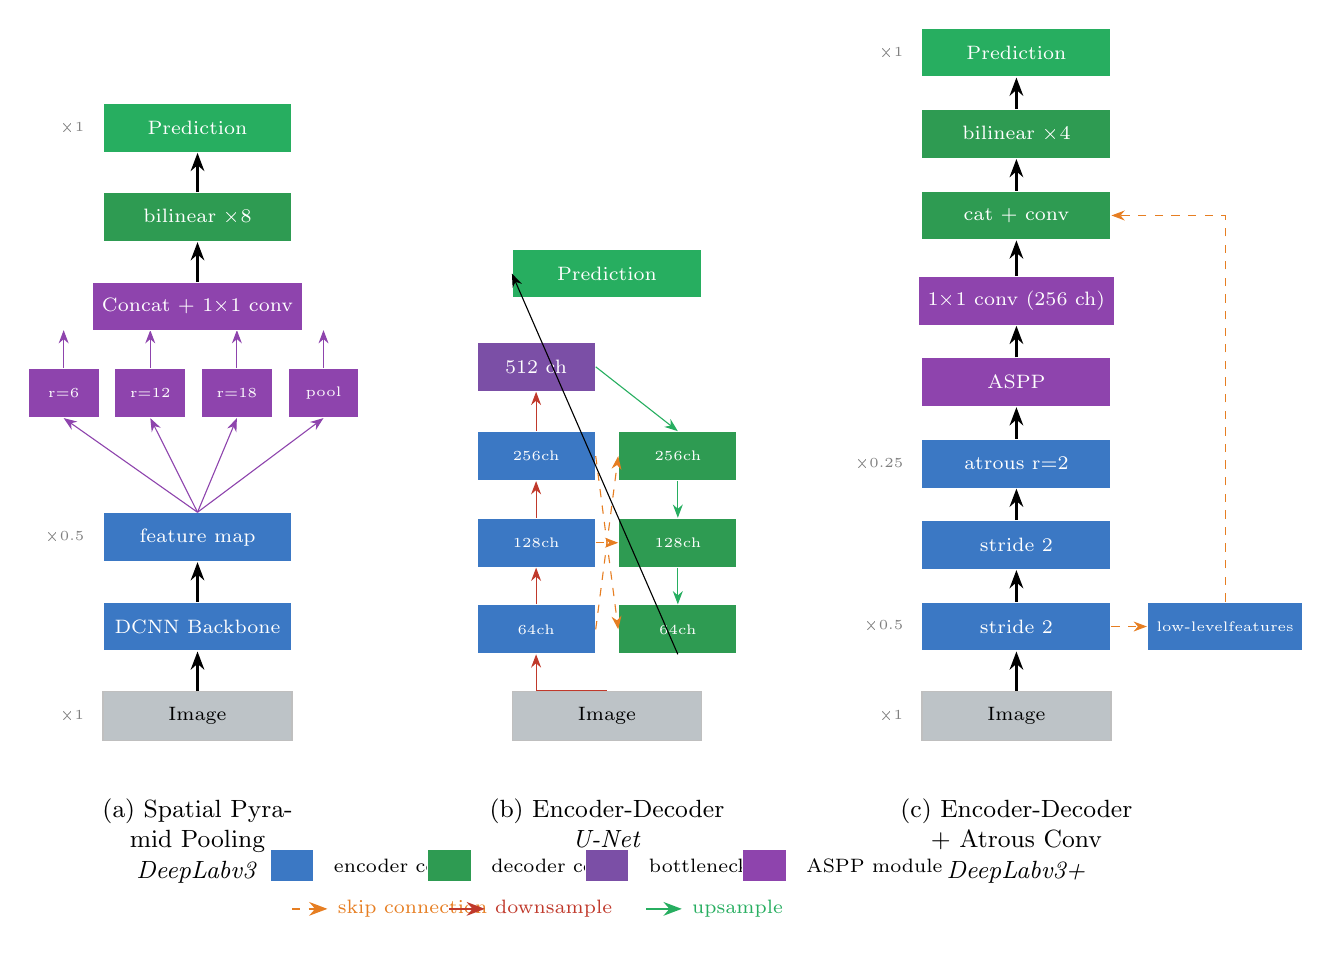
\begin{tikzpicture}[thick, node distance=0.55cm]

% Panel separation
\def\panelW{5.2}   % cm between panel centres

% ═══════════════════════════════════════════════════════════════════════════
% (a) Spatial Pyramid Pooling  [DeepLabv3]
% ═══════════════════════════════════════════════════════════════════════════
\begin{scope}[xshift=0cm]
  \def\cx{0}

  % Image
  \node[imgblk] (imgA) at (\cx, 0) {Image};

  % Backbone
  \node[blk=2.4cm, fill=cenc, above=0.5cm of imgA] (backA) {DCNN Backbone};
  \draw[->] (imgA.north) -- (backA.south);

  % Feature map
  \node[blk=2.4cm, fill=cenc, above=0.5cm of backA] (featA) {feature map};
  \draw[->] (backA.north) -- (featA.south);

  % ASPP branches: four boxes spread horizontally, connected with fan
  \foreach \i/\lbl in {1/r=6, 2/r=12, 3/r=18, 4/pool} {
    \pgfmathsetmacro{\bx}{\cx - 1.7 + (\i-1)*1.1}
    \node[blk=0.9cm, fill=caspp, font=\tiny]
      (aspp\i) at (\bx, 4.1) {\lbl};
    \draw[->, caspp, thin] (featA.north) -- (aspp\i.south);
    \draw[->, caspp, thin] (aspp\i.north) -- (\bx, 4.9);
  }

  % Concat
  \node[blk=2.4cm, fill=caspp] (catA) at (\cx, 5.2) {Concat + 1×1 conv};

  % Upsample
  \node[blk=2.4cm, fill=cdec, above=0.5cm of catA] (upA) {bilinear ×8};
  \draw[->] (catA.north) -- (upA.south);

  % Prediction
  \node[blk=2.4cm, fill=cpred, above=0.5cm of upA] (predA) {Prediction};
  \draw[->] (upA.north) -- (predA.south);

  % Scale labels (left side)
  \node[font=\tiny, gray, left=0.1cm of imgA]   {×1};
  \node[font=\tiny, gray, left=0.1cm of featA]  {×0.5};
  \node[font=\tiny, gray, left=0.1cm of predA]  {×1};

  % Caption
  \node[font=\small, below=0.6cm of imgA, text width=3cm, align=center]
    {(a) Spatial Pyramid Pooling\\\textit{DeepLabv3}};
\end{scope}

% ═══════════════════════════════════════════════════════════════════════════
% (b) Encoder-Decoder  [U-Net]
% ═══════════════════════════════════════════════════════════════════════════
\begin{scope}[xshift=\panelW cm]
  \def\cx{0}
  \def\exshift{-0.9}   % encoder column offset from cx
  \def\dxshift{ 0.9}   % decoder column offset from cx

  % Image
  \node[imgblk] (imgB) at (\cx, 0) {Image};

  % Encoder levels (going up = going deeper)
  \foreach \i/\ch in {1/64, 2/128, 3/256} {
    \pgfmathsetmacro{\yy}{\i * 1.1}
    \node[blk=1.5cm, fill=cenc, font=\tiny]
      (eB\i) at (\cx + \exshift, \yy) {\ch ch};
  }
  % Pool arrows between encoder levels
  \foreach \i in {1,2} {
    \pgfmathtruncatemacro{\j}{\i+1}
    \draw[->, cpool, thin] (eB\i.north) -- (eB\j.south);
  }
  \draw[->, cpool, thin] (imgB.north) -| (eB1.south);

  % Bottleneck
  \node[blk=1.5cm, fill=cbn, above=0.5cm of eB3] (bnB) {512 ch};
  \draw[->, cpool, thin] (eB3.north) -- (bnB.south);

  % Decoder levels (going up)
  \foreach \i/\ch in {1/256, 2/128, 3/64} {
    \pgfmathsetmacro{\yy}{(4-\i)*1.1}
    \node[blk=1.5cm, fill=cdec, font=\tiny]
      (dB\i) at (\cx + \dxshift, \yy) {\ch ch};
  }
  \draw[->, cup, thin] (bnB.east) -- (dB1.north);
  \foreach \i in {1,2} {
    \pgfmathtruncatemacro{\j}{\i+1}
    \draw[->, cup, thin] (dB\i.south) -- (dB\j.north);
  }

  % Skip connections
  \foreach \i in {1,2,3} {
    \draw[->, cskip, dashed, thin] (eB\i.east) -- (dB\i.west);
  }

  % Prediction
  \node[blk=2.4cm, fill=cpred, above=0.55cm of bnB, xshift=0.9cm]
    (predB) {Prediction};
  \draw[->, thin] (dB3.south) -- (predB.west);

  % Caption
  \node[font=\small, below=0.6cm of imgB, text width=3cm, align=center]
    {(b) Encoder-Decoder\\\textit{U-Net}};
\end{scope}

% ═══════════════════════════════════════════════════════════════════════════
% (c) Encoder-Decoder with Atrous Conv  [DeepLabv3+]
% ═══════════════════════════════════════════════════════════════════════════
\begin{scope}[xshift=2*\panelW cm]
  \def\cx{0}

  % Image
  \node[imgblk] (imgC) at (\cx, 0) {Image};

  % Encoder backbone (with atrous conv)
  \node[blk=2.4cm, fill=cenc, above=0.5cm of imgC]  (encC1) {stride 2};
  \node[blk=2.4cm, fill=cenc, above=0.4cm of encC1] (encC2) {stride 2};
  \node[blk=2.4cm, fill=cenc, above=0.4cm of encC2] (encC3) {atrous r=2};
  \draw[->] (imgC.north)  -- (encC1.south);
  \draw[->] (encC1.north) -- (encC2.south);
  \draw[->] (encC2.north) -- (encC3.south);

  % ASPP
  \node[blk=2.4cm, fill=caspp, above=0.4cm of encC3] (asppC) {ASPP};
  \draw[->] (encC3.north) -- (asppC.south);

  % 1×1 to reduce high-level features
  \node[blk=2.4cm, fill=caspp, above=0.4cm of asppC] (redC) {1×1 conv (256 ch)};
  \draw[->] (asppC.north) -- (redC.south);

  % Low-level feature (skip from early encoder)
  \node[blk=1.5cm, fill=cenc, font=\tiny,
        right=0.45cm of encC1] (llC) {low-level\\features};
  \draw[->, cskip, dashed, thin] (encC1.east) -- (llC.west);

  % Concat in decoder
  \node[blk=2.4cm, fill=cdec, above=0.45cm of redC] (catC) {cat + conv};
  \draw[->] (redC.north) -- (catC.south);
  \draw[->, cskip, dashed, thin] (llC.north) |- (catC.east);

  % Upsample + predict
  \node[blk=2.4cm, fill=cdec, above=0.4cm of catC] (upC) {bilinear ×4};
  \draw[->] (catC.north) -- (upC.south);
  \node[blk=2.4cm, fill=cpred, above=0.4cm of upC] (predC) {Prediction};
  \draw[->] (upC.north) -- (predC.south);

  % Scale labels
  \node[font=\tiny, gray, left=0.1cm of imgC]  {×1};
  \node[font=\tiny, gray, left=0.1cm of encC1] {×0.5};
  \node[font=\tiny, gray, left=0.1cm of encC3] {×0.25};
  \node[font=\tiny, gray, left=0.1cm of predC] {×1};

  % Caption
  \node[font=\small, below=0.6cm of imgC, text width=3.5cm, align=center]
    {(c) Encoder-Decoder + Atrous Conv\\\textit{DeepLabv3+}};
\end{scope}

% ── Shared legend (bottom, centred under all three panels) ─────────────────
\begin{scope}[shift={(\panelW, -1.9)}]
  \node[blk=0.55cm, fill=cenc,  minimum height=0.4cm] (lenc)  at (-4.0, 0) {};
  \node[right=0.12cm of lenc,  font=\scriptsize] {encoder conv};

  \node[blk=0.55cm, fill=cdec,  minimum height=0.4cm] (ldec)  at (-2.0, 0) {};
  \node[right=0.12cm of ldec,  font=\scriptsize] {decoder conv};

  \node[blk=0.55cm, fill=cbn,   minimum height=0.4cm] (lbn)   at ( 0.0, 0) {};
  \node[right=0.12cm of lbn,   font=\scriptsize] {bottleneck};

  \node[blk=0.55cm, fill=caspp, minimum height=0.4cm] (laspp) at ( 2.0, 0) {};
  \node[right=0.12cm of laspp, font=\scriptsize] {ASPP module};

  \draw[->, cskip, dashed] (-4.0, -0.55) -- ++( 0.45, 0)
    node[right, font=\scriptsize] {skip connection};
  \draw[->, cpool] (-2.0, -0.55) -- ++( 0.45, 0)
    node[right, font=\scriptsize] {downsample};
  \draw[->, cup]   ( 0.5, -0.55) -- ++( 0.45, 0)
    node[right, font=\scriptsize] {upsample};
\end{scope}

\end{tikzpicture}
\end{document}
